\section{Descrição do Problema}
O problema de decisão \textit{Grape Puzzle}, tal como descrito no site~\cite{ref_url1}, tem como objetivo, colocar um número positivo em cada "uva". Cada número na primeira linha tem apenas um dígito e nas restantes linhas, os números são a soma das duas "uvas" da linha imediatamente acima. Além disso, "uvas" com o mesmo número têm a mesma cor. Assim, podemos interpretar este problema como a resolução de \textit{n-1+...+1} somas, em que cores iguais representam variáveis iguais. Tomemos o exemplo, do problema seguinte, com 4 linhas:
\begin{figure}
    \centering
    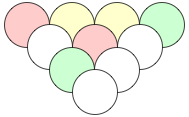
\includegraphics[scale=1]{problem.png}
    \caption{Problema de 4 Linhas}
    \label{fig: 4rowproblem}
\end{figure}

As somas correspondentes, apresentadas de linha a linha, serão:

\begin{equation}
    \systeme*{
    A \+ B = D  &\bigcap B \+ B = A  &\bigcap B \+ C = E ,
    D \+ A = C &\bigcap A \+ E = F,
    C \+ F = G
    }
\end{equation}

Tendo como solução:
\begin{figure}
    \centering
    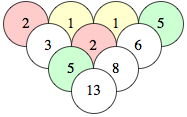
\includegraphics[scale=1]{solution.png}
    \caption{Solução de um problema de 4 Linhas}
    \label{fig: 4rowsolution}
\end{figure}